\documentclass[twoside]{book}

% Packages required by doxygen
\usepackage{fixltx2e}
\usepackage{calc}
\usepackage{doxygen}
\usepackage[export]{adjustbox} % also loads graphicx
\usepackage{graphicx}
\usepackage[utf8]{inputenc}
\usepackage{makeidx}
\usepackage{multicol}
\usepackage{multirow}
\PassOptionsToPackage{warn}{textcomp}
\usepackage{textcomp}
\usepackage[nointegrals]{wasysym}
\usepackage[table]{xcolor}

% Font selection
\usepackage[T1]{fontenc}
\usepackage[scaled=.90]{helvet}
\usepackage{courier}
\usepackage{amssymb}
\usepackage{sectsty}
\renewcommand{\familydefault}{\sfdefault}
\allsectionsfont{%
  \fontseries{bc}\selectfont%
  \color{darkgray}%
}
\renewcommand{\DoxyLabelFont}{%
  \fontseries{bc}\selectfont%
  \color{darkgray}%
}
\newcommand{\+}{\discretionary{\mbox{\scriptsize$\hookleftarrow$}}{}{}}

% Page & text layout
\usepackage{geometry}
\geometry{%
  a4paper,%
  top=2.5cm,%
  bottom=2.5cm,%
  left=2.5cm,%
  right=2.5cm%
}
\tolerance=750
\hfuzz=15pt
\hbadness=750
\setlength{\emergencystretch}{15pt}
\setlength{\parindent}{0cm}
\setlength{\parskip}{0.2cm}
\makeatletter
\renewcommand{\paragraph}{%
  \@startsection{paragraph}{4}{0ex}{-1.0ex}{1.0ex}{%
    \normalfont\normalsize\bfseries\SS@parafont%
  }%
}
\renewcommand{\subparagraph}{%
  \@startsection{subparagraph}{5}{0ex}{-1.0ex}{1.0ex}{%
    \normalfont\normalsize\bfseries\SS@subparafont%
  }%
}
\makeatother

% Headers & footers
\usepackage{fancyhdr}
\pagestyle{fancyplain}
\fancyhead[LE]{\fancyplain{}{\bfseries\thepage}}
\fancyhead[CE]{\fancyplain{}{}}
\fancyhead[RE]{\fancyplain{}{\bfseries\leftmark}}
\fancyhead[LO]{\fancyplain{}{\bfseries\rightmark}}
\fancyhead[CO]{\fancyplain{}{}}
\fancyhead[RO]{\fancyplain{}{\bfseries\thepage}}
\fancyfoot[LE]{\fancyplain{}{}}
\fancyfoot[CE]{\fancyplain{}{}}
\fancyfoot[RE]{\fancyplain{}{\bfseries\scriptsize Generated on Wed Apr 22 2015 19\+:15\+:40 for My Project by Doxygen }}
\fancyfoot[LO]{\fancyplain{}{\bfseries\scriptsize Generated on Wed Apr 22 2015 19\+:15\+:40 for My Project by Doxygen }}
\fancyfoot[CO]{\fancyplain{}{}}
\fancyfoot[RO]{\fancyplain{}{}}
\renewcommand{\footrulewidth}{0.4pt}
\renewcommand{\chaptermark}[1]{%
  \markboth{#1}{}%
}
\renewcommand{\sectionmark}[1]{%
  \markright{\thesection\ #1}%
}

% Indices & bibliography
\usepackage{natbib}
\usepackage[titles]{tocloft}
\setcounter{tocdepth}{3}
\setcounter{secnumdepth}{5}
\makeindex

% Hyperlinks (required, but should be loaded last)
\usepackage{ifpdf}
\ifpdf
  \usepackage[pdftex,pagebackref=true]{hyperref}
\else
  \usepackage[ps2pdf,pagebackref=true]{hyperref}
\fi
\hypersetup{%
  colorlinks=true,%
  linkcolor=blue,%
  citecolor=blue,%
  unicode%
}

% Custom commands
\newcommand{\clearemptydoublepage}{%
  \newpage{\pagestyle{empty}\cleardoublepage}%
}


%===== C O N T E N T S =====

\begin{document}

% Titlepage & ToC
\hypersetup{pageanchor=false,
             bookmarks=true,
             bookmarksnumbered=true,
             pdfencoding=unicode
            }
\pagenumbering{roman}
\begin{titlepage}
\vspace*{7cm}
\begin{center}%
{\Large My Project }\\
\vspace*{1cm}
{\large Generated by Doxygen 1.8.9.1}\\
\vspace*{0.5cm}
{\small Wed Apr 22 2015 19:15:40}\\
\end{center}
\end{titlepage}
\clearemptydoublepage
\tableofcontents
\clearemptydoublepage
\pagenumbering{arabic}
\hypersetup{pageanchor=true}

%--- Begin generated contents ---
\chapter{Hierarchical Index}
\section{Class Hierarchy}
This inheritance list is sorted roughly, but not completely, alphabetically\+:\begin{DoxyCompactList}
\item On\+Completion\+Listener\begin{DoxyCompactList}
\item \contentsline{section}{com.\+chopin.\+Music\+Service}{\pageref{classcom_1_1chopin_1_1MusicService}}{}
\end{DoxyCompactList}
\item On\+Double\+Tap\+Listener\begin{DoxyCompactList}
\item \contentsline{section}{com.\+chopin.\+Main\+Activity}{\pageref{classcom_1_1chopin_1_1MainActivity}}{}
\end{DoxyCompactList}
\item On\+Error\+Listener\begin{DoxyCompactList}
\item \contentsline{section}{com.\+chopin.\+Music\+Service}{\pageref{classcom_1_1chopin_1_1MusicService}}{}
\end{DoxyCompactList}
\item On\+Gesture\+Listener\begin{DoxyCompactList}
\item \contentsline{section}{com.\+chopin.\+Main\+Activity}{\pageref{classcom_1_1chopin_1_1MainActivity}}{}
\end{DoxyCompactList}
\item On\+Prepared\+Listener\begin{DoxyCompactList}
\item \contentsline{section}{com.\+chopin.\+Music\+Service}{\pageref{classcom_1_1chopin_1_1MusicService}}{}
\end{DoxyCompactList}
\item \contentsline{section}{com.\+chopin.\+Song}{\pageref{classcom_1_1chopin_1_1Song}}{}
\item Activity\begin{DoxyCompactList}
\item \contentsline{section}{com.\+chopin.\+Main\+Activity}{\pageref{classcom_1_1chopin_1_1MainActivity}}{}
\end{DoxyCompactList}
\item Base\+Adapter\begin{DoxyCompactList}
\item \contentsline{section}{com.\+chopin.\+Song\+Adapter}{\pageref{classcom_1_1chopin_1_1SongAdapter}}{}
\end{DoxyCompactList}
\item Binder\begin{DoxyCompactList}
\item \contentsline{section}{com.\+chopin.\+Music\+Service.\+Music\+Binder}{\pageref{classcom_1_1chopin_1_1MusicService_1_1MusicBinder}}{}
\end{DoxyCompactList}
\item Media\+Controller\begin{DoxyCompactList}
\item \contentsline{section}{com.\+chopin.\+Music\+Controller}{\pageref{classcom_1_1chopin_1_1MusicController}}{}
\end{DoxyCompactList}
\item Media\+Player\+Control\begin{DoxyCompactList}
\item \contentsline{section}{com.\+chopin.\+Main\+Activity}{\pageref{classcom_1_1chopin_1_1MainActivity}}{}
\end{DoxyCompactList}
\item Service\begin{DoxyCompactList}
\item \contentsline{section}{com.\+chopin.\+Music\+Service}{\pageref{classcom_1_1chopin_1_1MusicService}}{}
\end{DoxyCompactList}
\item Simple\+On\+Gesture\+Listener\begin{DoxyCompactList}
\item \contentsline{section}{com.\+chopin.\+Simple\+Gesture\+Filter}{\pageref{classcom_1_1chopin_1_1SimpleGestureFilter}}{}
\end{DoxyCompactList}
\end{DoxyCompactList}

\chapter{Class Index}
\section{Class List}
Here are the classes, structs, unions and interfaces with brief descriptions\+:\begin{DoxyCompactList}
\item\contentsline{section}{\hyperlink{classcom_1_1chopin_1_1MainActivity}{com.\+chopin.\+Main\+Activity} }{\pageref{classcom_1_1chopin_1_1MainActivity}}{}
\item\contentsline{section}{\hyperlink{classcom_1_1chopin_1_1MusicService_1_1MusicBinder}{com.\+chopin.\+Music\+Service.\+Music\+Binder} }{\pageref{classcom_1_1chopin_1_1MusicService_1_1MusicBinder}}{}
\item\contentsline{section}{\hyperlink{classcom_1_1chopin_1_1MusicController}{com.\+chopin.\+Music\+Controller} }{\pageref{classcom_1_1chopin_1_1MusicController}}{}
\item\contentsline{section}{\hyperlink{classcom_1_1chopin_1_1MusicService}{com.\+chopin.\+Music\+Service} }{\pageref{classcom_1_1chopin_1_1MusicService}}{}
\item\contentsline{section}{\hyperlink{classcom_1_1chopin_1_1SimpleGestureFilter}{com.\+chopin.\+Simple\+Gesture\+Filter} }{\pageref{classcom_1_1chopin_1_1SimpleGestureFilter}}{}
\item\contentsline{section}{\hyperlink{classcom_1_1chopin_1_1Song}{com.\+chopin.\+Song} }{\pageref{classcom_1_1chopin_1_1Song}}{}
\item\contentsline{section}{\hyperlink{classcom_1_1chopin_1_1SongAdapter}{com.\+chopin.\+Song\+Adapter} }{\pageref{classcom_1_1chopin_1_1SongAdapter}}{}
\end{DoxyCompactList}

\chapter{Class Documentation}
\hypertarget{classcom_1_1chopin_1_1MainActivity}{}\section{com.\+chopin.\+Main\+Activity Class Reference}
\label{classcom_1_1chopin_1_1MainActivity}\index{com.\+chopin.\+Main\+Activity@{com.\+chopin.\+Main\+Activity}}


Inheritance diagram for com.\+chopin.\+Main\+Activity\+:
\nopagebreak
\begin{figure}[H]
\begin{center}
\leavevmode
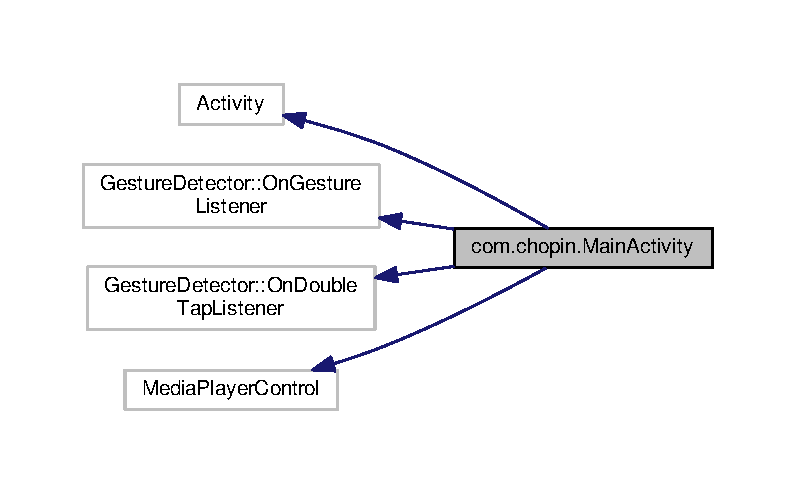
\includegraphics[width=350pt]{classcom_1_1chopin_1_1MainActivity__inherit__graph}
\end{center}
\end{figure}


Collaboration diagram for com.\+chopin.\+Main\+Activity\+:
\nopagebreak
\begin{figure}[H]
\begin{center}
\leavevmode
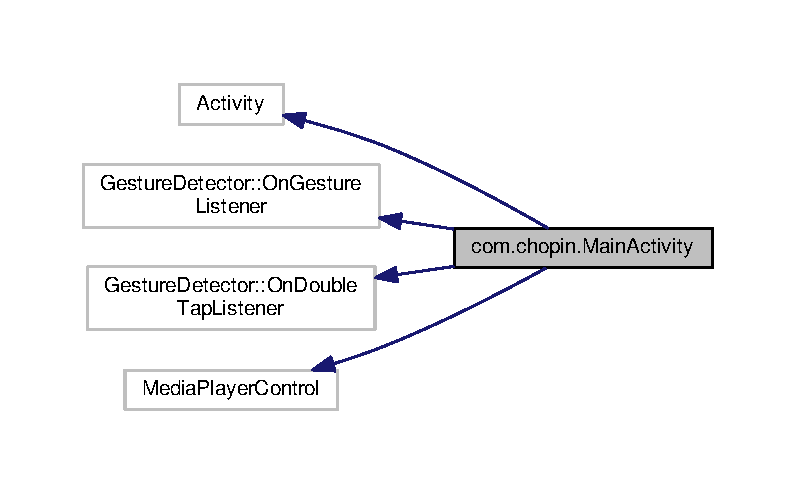
\includegraphics[width=350pt]{classcom_1_1chopin_1_1MainActivity__coll__graph}
\end{center}
\end{figure}
\subsection*{Public Member Functions}
\begin{DoxyCompactItemize}
\item 
boolean \hyperlink{classcom_1_1chopin_1_1MainActivity_a7ec09bc1bf1dcc68d369944ef5fed402}{on\+Touch\+Event} (Motion\+Event event)
\item 
boolean \hyperlink{classcom_1_1chopin_1_1MainActivity_ab5d46829409221b8219ac8b62532d913}{on\+Down} (Motion\+Event event)
\item 
boolean \hyperlink{classcom_1_1chopin_1_1MainActivity_a36c4ffe7e22d3f38f76fb983a360e220}{on\+Fling} (Motion\+Event event1, Motion\+Event event2, float velocity\+X, float velocity\+Y)
\item 
void \hyperlink{classcom_1_1chopin_1_1MainActivity_a447c24c7e4c1b41a0dc5c0d79b9ad7fe}{on\+Long\+Press} (Motion\+Event event)
\item 
boolean \hyperlink{classcom_1_1chopin_1_1MainActivity_aa76ce37b188dd077445f1aed639c2f13}{on\+Scroll} (Motion\+Event e1, Motion\+Event e2, float distance\+X, float distance\+Y)
\item 
void \hyperlink{classcom_1_1chopin_1_1MainActivity_aae7a255f30fa62752950d9c90d7e68b2}{on\+Show\+Press} (Motion\+Event event)
\item 
boolean \hyperlink{classcom_1_1chopin_1_1MainActivity_a128a997abbbee5a98a2898b0fe133bcc}{on\+Single\+Tap\+Up} (Motion\+Event event)
\item 
boolean \hyperlink{classcom_1_1chopin_1_1MainActivity_a09ebaf817b98ece078802a4506ac21e8}{on\+Double\+Tap} (Motion\+Event event)
\item 
boolean \hyperlink{classcom_1_1chopin_1_1MainActivity_a5a850938c326c53f4f7f9bed58c7d606}{on\+Double\+Tap\+Event} (Motion\+Event event)
\item 
boolean \hyperlink{classcom_1_1chopin_1_1MainActivity_afac4ea8c714deb0bb38f98f96d8d0752}{on\+Single\+Tap\+Confirmed} (Motion\+Event event)
\item 
boolean \hyperlink{classcom_1_1chopin_1_1MainActivity_adc17ea5ad991259ddeeeb7f7ba1e9e6c}{on\+Create\+Options\+Menu} (Menu menu)
\item 
boolean \hyperlink{classcom_1_1chopin_1_1MainActivity_a84a10910a3e427d8043dc84cf80b103d}{on\+Options\+Item\+Selected} (Menu\+Item item)
\item 
\hypertarget{classcom_1_1chopin_1_1MainActivity_a1d1874fbf0786331a959fdd2faafe693}{}void {\bfseries get\+Song\+List} ()\label{classcom_1_1chopin_1_1MainActivity_a1d1874fbf0786331a959fdd2faafe693}

\item 
\hypertarget{classcom_1_1chopin_1_1MainActivity_a3d12c6d0b2f85579ff3f3819dd37afd7}{}void {\bfseries start} ()\label{classcom_1_1chopin_1_1MainActivity_a3d12c6d0b2f85579ff3f3819dd37afd7}

\item 
\hypertarget{classcom_1_1chopin_1_1MainActivity_a83db75eb8bc461f4c54f3bf584604a04}{}void {\bfseries pause} ()\label{classcom_1_1chopin_1_1MainActivity_a83db75eb8bc461f4c54f3bf584604a04}

\item 
\hypertarget{classcom_1_1chopin_1_1MainActivity_abb7a64da3a10e19b6ac36da8dd35568d}{}int {\bfseries get\+Duration} ()\label{classcom_1_1chopin_1_1MainActivity_abb7a64da3a10e19b6ac36da8dd35568d}

\item 
\hypertarget{classcom_1_1chopin_1_1MainActivity_aa2c850e274f12487b6eaa0e3d52e726f}{}int {\bfseries get\+Current\+Position} ()\label{classcom_1_1chopin_1_1MainActivity_aa2c850e274f12487b6eaa0e3d52e726f}

\item 
\hypertarget{classcom_1_1chopin_1_1MainActivity_a0fc9bbd298406ea7562a0f7d566b4910}{}void {\bfseries seek\+To} (int pos)\label{classcom_1_1chopin_1_1MainActivity_a0fc9bbd298406ea7562a0f7d566b4910}

\item 
\hypertarget{classcom_1_1chopin_1_1MainActivity_abfa8d1fa01df8eab679a902045599472}{}boolean {\bfseries is\+Playing} ()\label{classcom_1_1chopin_1_1MainActivity_abfa8d1fa01df8eab679a902045599472}

\item 
\hypertarget{classcom_1_1chopin_1_1MainActivity_a95fd732ffa2aa7a90997fcf8220dc0f2}{}int {\bfseries get\+Buffer\+Percentage} ()\label{classcom_1_1chopin_1_1MainActivity_a95fd732ffa2aa7a90997fcf8220dc0f2}

\item 
\hypertarget{classcom_1_1chopin_1_1MainActivity_aba5b5949cb75c80c07e8213085b981bc}{}boolean {\bfseries can\+Pause} ()\label{classcom_1_1chopin_1_1MainActivity_aba5b5949cb75c80c07e8213085b981bc}

\item 
\hypertarget{classcom_1_1chopin_1_1MainActivity_a19e6c9effae33dea7432ec8abab0f4ae}{}boolean {\bfseries can\+Seek\+Backward} ()\label{classcom_1_1chopin_1_1MainActivity_a19e6c9effae33dea7432ec8abab0f4ae}

\item 
\hypertarget{classcom_1_1chopin_1_1MainActivity_ab3ea14cf52855a016133617257bbdb31}{}boolean {\bfseries can\+Seek\+Forward} ()\label{classcom_1_1chopin_1_1MainActivity_ab3ea14cf52855a016133617257bbdb31}

\item 
\hypertarget{classcom_1_1chopin_1_1MainActivity_a0b28aa1b5dd82709c3ff610be90a0fe6}{}int {\bfseries get\+Audio\+Session\+Id} ()\label{classcom_1_1chopin_1_1MainActivity_a0b28aa1b5dd82709c3ff610be90a0fe6}

\item 
void \hyperlink{classcom_1_1chopin_1_1MainActivity_a9f4a1395a15719ded6774bf85aa03bcb}{song\+Picked} (View view)
\end{DoxyCompactItemize}
\subsection*{Protected Member Functions}
\begin{DoxyCompactItemize}
\item 
void \hyperlink{classcom_1_1chopin_1_1MainActivity_af3b282552cb382d8569a2f440633270a}{on\+Create} (Bundle saved\+Instance\+State)
\item 
\hypertarget{classcom_1_1chopin_1_1MainActivity_a999cb3456369f7234fc3e7a26f5952ec}{}void {\bfseries on\+Start} ()\label{classcom_1_1chopin_1_1MainActivity_a999cb3456369f7234fc3e7a26f5952ec}

\item 
\hypertarget{classcom_1_1chopin_1_1MainActivity_a75a68c1f77d4c550c5aee79774b70104}{}void {\bfseries on\+Destroy} ()\label{classcom_1_1chopin_1_1MainActivity_a75a68c1f77d4c550c5aee79774b70104}

\item 
\hypertarget{classcom_1_1chopin_1_1MainActivity_aeb4448efd5f2523306ba3245f2346be4}{}void {\bfseries on\+Pause} ()\label{classcom_1_1chopin_1_1MainActivity_aeb4448efd5f2523306ba3245f2346be4}

\item 
\hypertarget{classcom_1_1chopin_1_1MainActivity_a9e8e5a906b0ea0012db4134aeae6da83}{}void {\bfseries on\+Resume} ()\label{classcom_1_1chopin_1_1MainActivity_a9e8e5a906b0ea0012db4134aeae6da83}

\item 
\hypertarget{classcom_1_1chopin_1_1MainActivity_aed63ff8097276b312fb8a6a29a3f3266}{}void {\bfseries on\+Stop} ()\label{classcom_1_1chopin_1_1MainActivity_aed63ff8097276b312fb8a6a29a3f3266}

\end{DoxyCompactItemize}


\subsection{Member Function Documentation}
\hypertarget{classcom_1_1chopin_1_1MainActivity_af3b282552cb382d8569a2f440633270a}{}\index{com\+::chopin\+::\+Main\+Activity@{com\+::chopin\+::\+Main\+Activity}!on\+Create@{on\+Create}}
\index{on\+Create@{on\+Create}!com\+::chopin\+::\+Main\+Activity@{com\+::chopin\+::\+Main\+Activity}}
\subsubsection[{on\+Create}]{\setlength{\rightskip}{0pt plus 5cm}void com.\+chopin.\+Main\+Activity.\+on\+Create (
\begin{DoxyParamCaption}
\item[{Bundle}]{saved\+Instance\+State}
\end{DoxyParamCaption}
)\hspace{0.3cm}{\ttfamily [inline]}, {\ttfamily [protected]}}\label{classcom_1_1chopin_1_1MainActivity_af3b282552cb382d8569a2f440633270a}

\begin{DoxyParams}{Parameters}
{\em saved\+Instance\+State} & \\
\hline
\end{DoxyParams}
\hypertarget{classcom_1_1chopin_1_1MainActivity_adc17ea5ad991259ddeeeb7f7ba1e9e6c}{}\index{com\+::chopin\+::\+Main\+Activity@{com\+::chopin\+::\+Main\+Activity}!on\+Create\+Options\+Menu@{on\+Create\+Options\+Menu}}
\index{on\+Create\+Options\+Menu@{on\+Create\+Options\+Menu}!com\+::chopin\+::\+Main\+Activity@{com\+::chopin\+::\+Main\+Activity}}
\subsubsection[{on\+Create\+Options\+Menu}]{\setlength{\rightskip}{0pt plus 5cm}boolean com.\+chopin.\+Main\+Activity.\+on\+Create\+Options\+Menu (
\begin{DoxyParamCaption}
\item[{Menu}]{menu}
\end{DoxyParamCaption}
)\hspace{0.3cm}{\ttfamily [inline]}}\label{classcom_1_1chopin_1_1MainActivity_adc17ea5ad991259ddeeeb7f7ba1e9e6c}

\begin{DoxyParams}{Parameters}
{\em menu} & \\
\hline
\end{DoxyParams}
\begin{DoxyReturn}{Returns}

\end{DoxyReturn}
\hypertarget{classcom_1_1chopin_1_1MainActivity_a09ebaf817b98ece078802a4506ac21e8}{}\index{com\+::chopin\+::\+Main\+Activity@{com\+::chopin\+::\+Main\+Activity}!on\+Double\+Tap@{on\+Double\+Tap}}
\index{on\+Double\+Tap@{on\+Double\+Tap}!com\+::chopin\+::\+Main\+Activity@{com\+::chopin\+::\+Main\+Activity}}
\subsubsection[{on\+Double\+Tap}]{\setlength{\rightskip}{0pt plus 5cm}boolean com.\+chopin.\+Main\+Activity.\+on\+Double\+Tap (
\begin{DoxyParamCaption}
\item[{Motion\+Event}]{event}
\end{DoxyParamCaption}
)\hspace{0.3cm}{\ttfamily [inline]}}\label{classcom_1_1chopin_1_1MainActivity_a09ebaf817b98ece078802a4506ac21e8}

\begin{DoxyParams}{Parameters}
{\em event} & \\
\hline
\end{DoxyParams}
\begin{DoxyReturn}{Returns}

\end{DoxyReturn}
\hypertarget{classcom_1_1chopin_1_1MainActivity_a5a850938c326c53f4f7f9bed58c7d606}{}\index{com\+::chopin\+::\+Main\+Activity@{com\+::chopin\+::\+Main\+Activity}!on\+Double\+Tap\+Event@{on\+Double\+Tap\+Event}}
\index{on\+Double\+Tap\+Event@{on\+Double\+Tap\+Event}!com\+::chopin\+::\+Main\+Activity@{com\+::chopin\+::\+Main\+Activity}}
\subsubsection[{on\+Double\+Tap\+Event}]{\setlength{\rightskip}{0pt plus 5cm}boolean com.\+chopin.\+Main\+Activity.\+on\+Double\+Tap\+Event (
\begin{DoxyParamCaption}
\item[{Motion\+Event}]{event}
\end{DoxyParamCaption}
)\hspace{0.3cm}{\ttfamily [inline]}}\label{classcom_1_1chopin_1_1MainActivity_a5a850938c326c53f4f7f9bed58c7d606}

\begin{DoxyParams}{Parameters}
{\em event} & \\
\hline
\end{DoxyParams}
\begin{DoxyReturn}{Returns}

\end{DoxyReturn}
\hypertarget{classcom_1_1chopin_1_1MainActivity_ab5d46829409221b8219ac8b62532d913}{}\index{com\+::chopin\+::\+Main\+Activity@{com\+::chopin\+::\+Main\+Activity}!on\+Down@{on\+Down}}
\index{on\+Down@{on\+Down}!com\+::chopin\+::\+Main\+Activity@{com\+::chopin\+::\+Main\+Activity}}
\subsubsection[{on\+Down}]{\setlength{\rightskip}{0pt plus 5cm}boolean com.\+chopin.\+Main\+Activity.\+on\+Down (
\begin{DoxyParamCaption}
\item[{Motion\+Event}]{event}
\end{DoxyParamCaption}
)\hspace{0.3cm}{\ttfamily [inline]}}\label{classcom_1_1chopin_1_1MainActivity_ab5d46829409221b8219ac8b62532d913}

\begin{DoxyParams}{Parameters}
{\em event} & \\
\hline
\end{DoxyParams}
\begin{DoxyReturn}{Returns}

\end{DoxyReturn}
\hypertarget{classcom_1_1chopin_1_1MainActivity_a36c4ffe7e22d3f38f76fb983a360e220}{}\index{com\+::chopin\+::\+Main\+Activity@{com\+::chopin\+::\+Main\+Activity}!on\+Fling@{on\+Fling}}
\index{on\+Fling@{on\+Fling}!com\+::chopin\+::\+Main\+Activity@{com\+::chopin\+::\+Main\+Activity}}
\subsubsection[{on\+Fling}]{\setlength{\rightskip}{0pt plus 5cm}boolean com.\+chopin.\+Main\+Activity.\+on\+Fling (
\begin{DoxyParamCaption}
\item[{Motion\+Event}]{event1, }
\item[{Motion\+Event}]{event2, }
\item[{float}]{velocity\+X, }
\item[{float}]{velocity\+Y}
\end{DoxyParamCaption}
)\hspace{0.3cm}{\ttfamily [inline]}}\label{classcom_1_1chopin_1_1MainActivity_a36c4ffe7e22d3f38f76fb983a360e220}

\begin{DoxyParams}{Parameters}
{\em event1} & \\
\hline
{\em event2} & \\
\hline
{\em velocity\+X} & \\
\hline
{\em velocity\+Y} & \\
\hline
\end{DoxyParams}
\begin{DoxyReturn}{Returns}

\end{DoxyReturn}
\hypertarget{classcom_1_1chopin_1_1MainActivity_a447c24c7e4c1b41a0dc5c0d79b9ad7fe}{}\index{com\+::chopin\+::\+Main\+Activity@{com\+::chopin\+::\+Main\+Activity}!on\+Long\+Press@{on\+Long\+Press}}
\index{on\+Long\+Press@{on\+Long\+Press}!com\+::chopin\+::\+Main\+Activity@{com\+::chopin\+::\+Main\+Activity}}
\subsubsection[{on\+Long\+Press}]{\setlength{\rightskip}{0pt plus 5cm}void com.\+chopin.\+Main\+Activity.\+on\+Long\+Press (
\begin{DoxyParamCaption}
\item[{Motion\+Event}]{event}
\end{DoxyParamCaption}
)\hspace{0.3cm}{\ttfamily [inline]}}\label{classcom_1_1chopin_1_1MainActivity_a447c24c7e4c1b41a0dc5c0d79b9ad7fe}

\begin{DoxyParams}{Parameters}
{\em event} & \\
\hline
\end{DoxyParams}
\hypertarget{classcom_1_1chopin_1_1MainActivity_a84a10910a3e427d8043dc84cf80b103d}{}\index{com\+::chopin\+::\+Main\+Activity@{com\+::chopin\+::\+Main\+Activity}!on\+Options\+Item\+Selected@{on\+Options\+Item\+Selected}}
\index{on\+Options\+Item\+Selected@{on\+Options\+Item\+Selected}!com\+::chopin\+::\+Main\+Activity@{com\+::chopin\+::\+Main\+Activity}}
\subsubsection[{on\+Options\+Item\+Selected}]{\setlength{\rightskip}{0pt plus 5cm}boolean com.\+chopin.\+Main\+Activity.\+on\+Options\+Item\+Selected (
\begin{DoxyParamCaption}
\item[{Menu\+Item}]{item}
\end{DoxyParamCaption}
)\hspace{0.3cm}{\ttfamily [inline]}}\label{classcom_1_1chopin_1_1MainActivity_a84a10910a3e427d8043dc84cf80b103d}

\begin{DoxyParams}{Parameters}
{\em item} & \\
\hline
\end{DoxyParams}
\begin{DoxyReturn}{Returns}

\end{DoxyReturn}
\hypertarget{classcom_1_1chopin_1_1MainActivity_aa76ce37b188dd077445f1aed639c2f13}{}\index{com\+::chopin\+::\+Main\+Activity@{com\+::chopin\+::\+Main\+Activity}!on\+Scroll@{on\+Scroll}}
\index{on\+Scroll@{on\+Scroll}!com\+::chopin\+::\+Main\+Activity@{com\+::chopin\+::\+Main\+Activity}}
\subsubsection[{on\+Scroll}]{\setlength{\rightskip}{0pt plus 5cm}boolean com.\+chopin.\+Main\+Activity.\+on\+Scroll (
\begin{DoxyParamCaption}
\item[{Motion\+Event}]{e1, }
\item[{Motion\+Event}]{e2, }
\item[{float}]{distance\+X, }
\item[{float}]{distance\+Y}
\end{DoxyParamCaption}
)\hspace{0.3cm}{\ttfamily [inline]}}\label{classcom_1_1chopin_1_1MainActivity_aa76ce37b188dd077445f1aed639c2f13}

\begin{DoxyParams}{Parameters}
{\em e1} & \\
\hline
{\em e2} & \\
\hline
{\em distance\+X} & \\
\hline
{\em distance\+Y} & \\
\hline
\end{DoxyParams}
\begin{DoxyReturn}{Returns}

\end{DoxyReturn}
\hypertarget{classcom_1_1chopin_1_1MainActivity_aae7a255f30fa62752950d9c90d7e68b2}{}\index{com\+::chopin\+::\+Main\+Activity@{com\+::chopin\+::\+Main\+Activity}!on\+Show\+Press@{on\+Show\+Press}}
\index{on\+Show\+Press@{on\+Show\+Press}!com\+::chopin\+::\+Main\+Activity@{com\+::chopin\+::\+Main\+Activity}}
\subsubsection[{on\+Show\+Press}]{\setlength{\rightskip}{0pt plus 5cm}void com.\+chopin.\+Main\+Activity.\+on\+Show\+Press (
\begin{DoxyParamCaption}
\item[{Motion\+Event}]{event}
\end{DoxyParamCaption}
)\hspace{0.3cm}{\ttfamily [inline]}}\label{classcom_1_1chopin_1_1MainActivity_aae7a255f30fa62752950d9c90d7e68b2}

\begin{DoxyParams}{Parameters}
{\em event} & \\
\hline
\end{DoxyParams}
\hypertarget{classcom_1_1chopin_1_1MainActivity_afac4ea8c714deb0bb38f98f96d8d0752}{}\index{com\+::chopin\+::\+Main\+Activity@{com\+::chopin\+::\+Main\+Activity}!on\+Single\+Tap\+Confirmed@{on\+Single\+Tap\+Confirmed}}
\index{on\+Single\+Tap\+Confirmed@{on\+Single\+Tap\+Confirmed}!com\+::chopin\+::\+Main\+Activity@{com\+::chopin\+::\+Main\+Activity}}
\subsubsection[{on\+Single\+Tap\+Confirmed}]{\setlength{\rightskip}{0pt plus 5cm}boolean com.\+chopin.\+Main\+Activity.\+on\+Single\+Tap\+Confirmed (
\begin{DoxyParamCaption}
\item[{Motion\+Event}]{event}
\end{DoxyParamCaption}
)\hspace{0.3cm}{\ttfamily [inline]}}\label{classcom_1_1chopin_1_1MainActivity_afac4ea8c714deb0bb38f98f96d8d0752}

\begin{DoxyParams}{Parameters}
{\em event} & \\
\hline
\end{DoxyParams}
\begin{DoxyReturn}{Returns}

\end{DoxyReturn}
\hypertarget{classcom_1_1chopin_1_1MainActivity_a128a997abbbee5a98a2898b0fe133bcc}{}\index{com\+::chopin\+::\+Main\+Activity@{com\+::chopin\+::\+Main\+Activity}!on\+Single\+Tap\+Up@{on\+Single\+Tap\+Up}}
\index{on\+Single\+Tap\+Up@{on\+Single\+Tap\+Up}!com\+::chopin\+::\+Main\+Activity@{com\+::chopin\+::\+Main\+Activity}}
\subsubsection[{on\+Single\+Tap\+Up}]{\setlength{\rightskip}{0pt plus 5cm}boolean com.\+chopin.\+Main\+Activity.\+on\+Single\+Tap\+Up (
\begin{DoxyParamCaption}
\item[{Motion\+Event}]{event}
\end{DoxyParamCaption}
)\hspace{0.3cm}{\ttfamily [inline]}}\label{classcom_1_1chopin_1_1MainActivity_a128a997abbbee5a98a2898b0fe133bcc}

\begin{DoxyParams}{Parameters}
{\em event} & \\
\hline
\end{DoxyParams}
\begin{DoxyReturn}{Returns}

\end{DoxyReturn}
\hypertarget{classcom_1_1chopin_1_1MainActivity_a7ec09bc1bf1dcc68d369944ef5fed402}{}\index{com\+::chopin\+::\+Main\+Activity@{com\+::chopin\+::\+Main\+Activity}!on\+Touch\+Event@{on\+Touch\+Event}}
\index{on\+Touch\+Event@{on\+Touch\+Event}!com\+::chopin\+::\+Main\+Activity@{com\+::chopin\+::\+Main\+Activity}}
\subsubsection[{on\+Touch\+Event}]{\setlength{\rightskip}{0pt plus 5cm}boolean com.\+chopin.\+Main\+Activity.\+on\+Touch\+Event (
\begin{DoxyParamCaption}
\item[{Motion\+Event}]{event}
\end{DoxyParamCaption}
)\hspace{0.3cm}{\ttfamily [inline]}}\label{classcom_1_1chopin_1_1MainActivity_a7ec09bc1bf1dcc68d369944ef5fed402}

\begin{DoxyParams}{Parameters}
{\em event} & \\
\hline
\end{DoxyParams}
\begin{DoxyReturn}{Returns}

\end{DoxyReturn}
\hypertarget{classcom_1_1chopin_1_1MainActivity_a9f4a1395a15719ded6774bf85aa03bcb}{}\index{com\+::chopin\+::\+Main\+Activity@{com\+::chopin\+::\+Main\+Activity}!song\+Picked@{song\+Picked}}
\index{song\+Picked@{song\+Picked}!com\+::chopin\+::\+Main\+Activity@{com\+::chopin\+::\+Main\+Activity}}
\subsubsection[{song\+Picked}]{\setlength{\rightskip}{0pt plus 5cm}void com.\+chopin.\+Main\+Activity.\+song\+Picked (
\begin{DoxyParamCaption}
\item[{View}]{view}
\end{DoxyParamCaption}
)\hspace{0.3cm}{\ttfamily [inline]}}\label{classcom_1_1chopin_1_1MainActivity_a9f4a1395a15719ded6774bf85aa03bcb}

\begin{DoxyParams}{Parameters}
{\em view} & \\
\hline
\end{DoxyParams}


The documentation for this class was generated from the following file\+:\begin{DoxyCompactItemize}
\item 
Main\+Activity.\+java\end{DoxyCompactItemize}

\hypertarget{classcom_1_1chopin_1_1MusicService_1_1MusicBinder}{}\section{com.\+chopin.\+Music\+Service.\+Music\+Binder Class Reference}
\label{classcom_1_1chopin_1_1MusicService_1_1MusicBinder}\index{com.\+chopin.\+Music\+Service.\+Music\+Binder@{com.\+chopin.\+Music\+Service.\+Music\+Binder}}


Inheritance diagram for com.\+chopin.\+Music\+Service.\+Music\+Binder\+:
\nopagebreak
\begin{figure}[H]
\begin{center}
\leavevmode
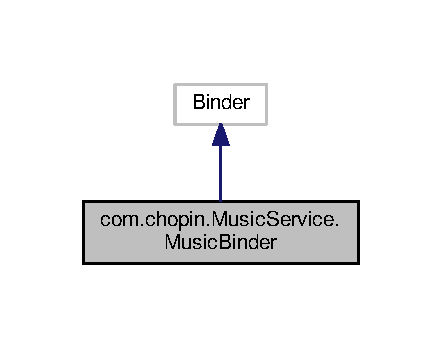
\includegraphics[width=212pt]{classcom_1_1chopin_1_1MusicService_1_1MusicBinder__inherit__graph}
\end{center}
\end{figure}


Collaboration diagram for com.\+chopin.\+Music\+Service.\+Music\+Binder\+:
\nopagebreak
\begin{figure}[H]
\begin{center}
\leavevmode
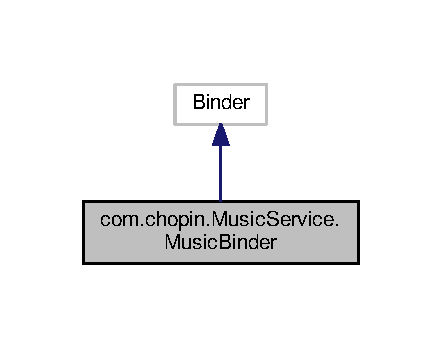
\includegraphics[width=212pt]{classcom_1_1chopin_1_1MusicService_1_1MusicBinder__coll__graph}
\end{center}
\end{figure}


The documentation for this class was generated from the following file\+:\begin{DoxyCompactItemize}
\item 
Music\+Service.\+java\end{DoxyCompactItemize}

\hypertarget{classcom_1_1chopin_1_1MusicController}{}\section{com.\+chopin.\+Music\+Controller Class Reference}
\label{classcom_1_1chopin_1_1MusicController}\index{com.\+chopin.\+Music\+Controller@{com.\+chopin.\+Music\+Controller}}


Inheritance diagram for com.\+chopin.\+Music\+Controller\+:
\nopagebreak
\begin{figure}[H]
\begin{center}
\leavevmode
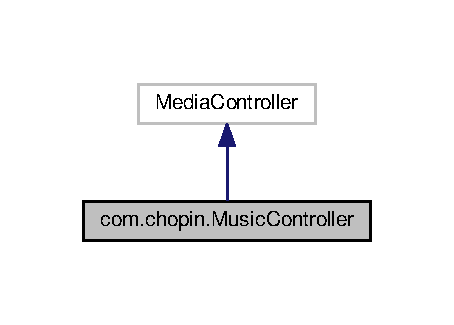
\includegraphics[width=218pt]{classcom_1_1chopin_1_1MusicController__inherit__graph}
\end{center}
\end{figure}


Collaboration diagram for com.\+chopin.\+Music\+Controller\+:
\nopagebreak
\begin{figure}[H]
\begin{center}
\leavevmode
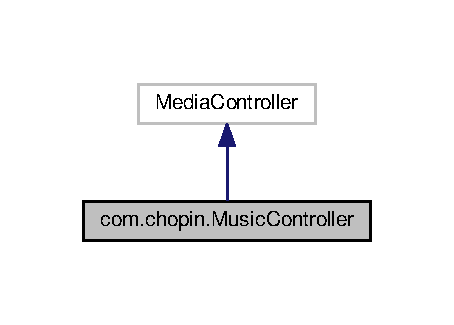
\includegraphics[width=218pt]{classcom_1_1chopin_1_1MusicController__coll__graph}
\end{center}
\end{figure}
\subsection*{Public Member Functions}
\begin{DoxyCompactItemize}
\item 
\hypertarget{classcom_1_1chopin_1_1MusicController_a3f68f15cba5ad8a85ee59b54501f1e84}{}{\bfseries Music\+Controller} (Context c)\label{classcom_1_1chopin_1_1MusicController_a3f68f15cba5ad8a85ee59b54501f1e84}

\item 
\hypertarget{classcom_1_1chopin_1_1MusicController_ae50a2139682ad573643ddfd21aee6a54}{}void {\bfseries hide} ()\label{classcom_1_1chopin_1_1MusicController_ae50a2139682ad573643ddfd21aee6a54}

\end{DoxyCompactItemize}


\subsection{Detailed Description}
Created by branden on 3/4/15. 

The documentation for this class was generated from the following file\+:\begin{DoxyCompactItemize}
\item 
Music\+Controller.\+java\end{DoxyCompactItemize}

\hypertarget{classcom_1_1chopin_1_1MusicService}{}\section{com.\+chopin.\+Music\+Service Class Reference}
\label{classcom_1_1chopin_1_1MusicService}\index{com.\+chopin.\+Music\+Service@{com.\+chopin.\+Music\+Service}}


Inheritance diagram for com.\+chopin.\+Music\+Service\+:\nopagebreak
\begin{figure}[H]
\begin{center}
\leavevmode
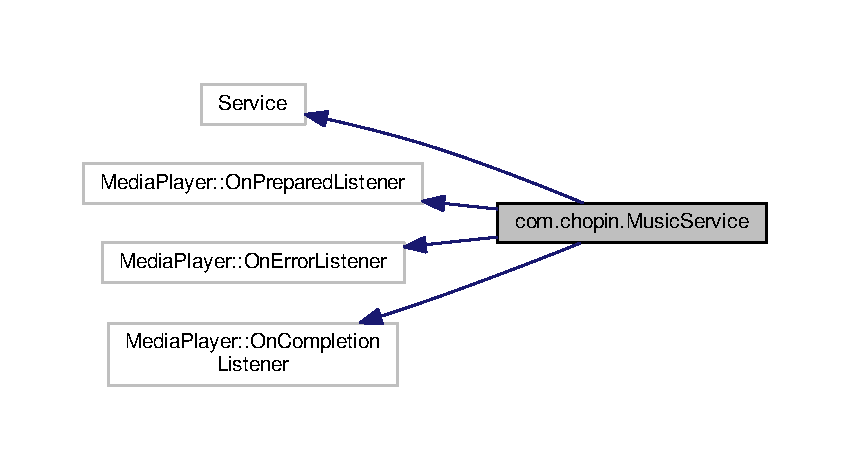
\includegraphics[width=350pt]{classcom_1_1chopin_1_1MusicService__inherit__graph}
\end{center}
\end{figure}


Collaboration diagram for com.\+chopin.\+Music\+Service\+:\nopagebreak
\begin{figure}[H]
\begin{center}
\leavevmode
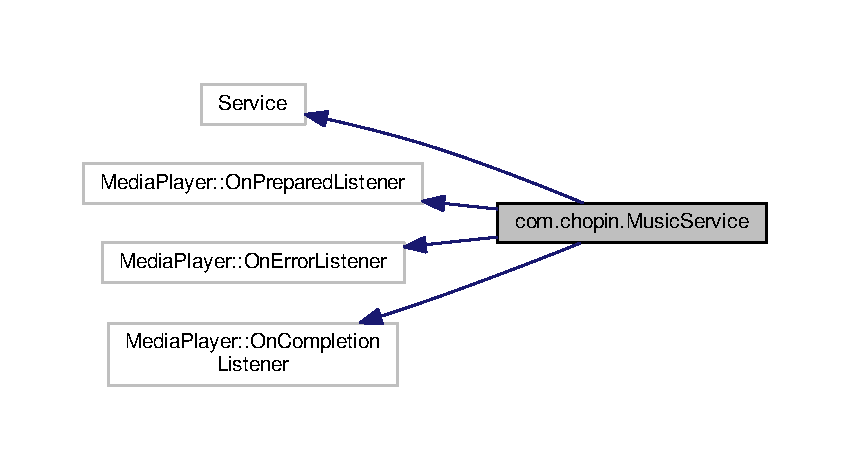
\includegraphics[width=350pt]{classcom_1_1chopin_1_1MusicService__coll__graph}
\end{center}
\end{figure}
\subsection*{Classes}
\begin{DoxyCompactItemize}
\item 
class \hyperlink{classcom_1_1chopin_1_1MusicService_1_1MusicBinder}{Music\+Binder}
\end{DoxyCompactItemize}
\subsection*{Public Member Functions}
\begin{DoxyCompactItemize}
\item 
\hypertarget{classcom_1_1chopin_1_1MusicService_aa1ff15c5f6f8be8e776ed950e9c0df7c}{}void {\bfseries on\+Create} ()\label{classcom_1_1chopin_1_1MusicService_aa1ff15c5f6f8be8e776ed950e9c0df7c}

\item 
\hypertarget{classcom_1_1chopin_1_1MusicService_acf884fbbfba22327e684c7f1bbc9a680}{}void {\bfseries init\+Music\+Player} ()\label{classcom_1_1chopin_1_1MusicService_acf884fbbfba22327e684c7f1bbc9a680}

\item 
\hypertarget{classcom_1_1chopin_1_1MusicService_ad5b53ad2e0130fa4f1378a57820a2b32}{}void {\bfseries set\+List} (Array\+List$<$ \hyperlink{classcom_1_1chopin_1_1Song}{Song} $>$ the\+Songs)\label{classcom_1_1chopin_1_1MusicService_ad5b53ad2e0130fa4f1378a57820a2b32}

\item 
\hypertarget{classcom_1_1chopin_1_1MusicService_ace5083ece383284817ee86ad52cbadfd}{}I\+Binder {\bfseries on\+Bind} (Intent arg0)\label{classcom_1_1chopin_1_1MusicService_ace5083ece383284817ee86ad52cbadfd}

\item 
\hypertarget{classcom_1_1chopin_1_1MusicService_a0bfdf09a4912089254e7d9bcca31a5c3}{}boolean {\bfseries on\+Unbind} (Intent intent)\label{classcom_1_1chopin_1_1MusicService_a0bfdf09a4912089254e7d9bcca31a5c3}

\item 
\hypertarget{classcom_1_1chopin_1_1MusicService_acb6e4da174fdadfbbf09e06fb7144db4}{}void {\bfseries on\+Completion} (Media\+Player mp)\label{classcom_1_1chopin_1_1MusicService_acb6e4da174fdadfbbf09e06fb7144db4}

\item 
\hypertarget{classcom_1_1chopin_1_1MusicService_ad2e786c061d8f06800a3c93a2496dac6}{}boolean {\bfseries on\+Error} (Media\+Player mp, int what, int extra)\label{classcom_1_1chopin_1_1MusicService_ad2e786c061d8f06800a3c93a2496dac6}

\item 
\hypertarget{classcom_1_1chopin_1_1MusicService_a1f4838d19b85ccff29c3bf1c9548efcf}{}void {\bfseries on\+Prepared} (Media\+Player mp)\label{classcom_1_1chopin_1_1MusicService_a1f4838d19b85ccff29c3bf1c9548efcf}

\item 
\hypertarget{classcom_1_1chopin_1_1MusicService_a68f5b20ddc76bc2135bbcf23fd50e3cf}{}void {\bfseries set\+Song} (int song\+Index)\label{classcom_1_1chopin_1_1MusicService_a68f5b20ddc76bc2135bbcf23fd50e3cf}

\item 
\hypertarget{classcom_1_1chopin_1_1MusicService_a7168cc0a3235589ba228b79664ac3164}{}void {\bfseries play\+Song} ()\label{classcom_1_1chopin_1_1MusicService_a7168cc0a3235589ba228b79664ac3164}

\item 
\hypertarget{classcom_1_1chopin_1_1MusicService_abda19226556fedb7153968f397ce6c15}{}int {\bfseries get\+Posn} ()\label{classcom_1_1chopin_1_1MusicService_abda19226556fedb7153968f397ce6c15}

\item 
\hypertarget{classcom_1_1chopin_1_1MusicService_aa8b9e5ec39463320bd9b32e822f91524}{}int {\bfseries get\+Dur} ()\label{classcom_1_1chopin_1_1MusicService_aa8b9e5ec39463320bd9b32e822f91524}

\item 
\hypertarget{classcom_1_1chopin_1_1MusicService_a929dc1f0780af460625b5638e264f269}{}boolean {\bfseries is\+Png} ()\label{classcom_1_1chopin_1_1MusicService_a929dc1f0780af460625b5638e264f269}

\item 
\hypertarget{classcom_1_1chopin_1_1MusicService_a1858327c8f552e1b069a068ef8686933}{}void {\bfseries pause\+Player} ()\label{classcom_1_1chopin_1_1MusicService_a1858327c8f552e1b069a068ef8686933}

\item 
\hypertarget{classcom_1_1chopin_1_1MusicService_ab32e202b783e666b28eca034019f0964}{}void {\bfseries seek} (int posn)\label{classcom_1_1chopin_1_1MusicService_ab32e202b783e666b28eca034019f0964}

\item 
\hypertarget{classcom_1_1chopin_1_1MusicService_a6f8ab60cbf202c51af64877bd7c4a75e}{}void {\bfseries go} ()\label{classcom_1_1chopin_1_1MusicService_a6f8ab60cbf202c51af64877bd7c4a75e}

\item 
\hypertarget{classcom_1_1chopin_1_1MusicService_adf931c14f29fec1aec415b09c9b076aa}{}void {\bfseries play\+Prev} ()\label{classcom_1_1chopin_1_1MusicService_adf931c14f29fec1aec415b09c9b076aa}

\item 
\hypertarget{classcom_1_1chopin_1_1MusicService_aac03a796c882bd43e9ef1fad426be8ca}{}void {\bfseries play\+Next} ()\label{classcom_1_1chopin_1_1MusicService_aac03a796c882bd43e9ef1fad426be8ca}

\item 
\hypertarget{classcom_1_1chopin_1_1MusicService_a223dae031fa16712469118165bb3daa9}{}void {\bfseries on\+Destroy} ()\label{classcom_1_1chopin_1_1MusicService_a223dae031fa16712469118165bb3daa9}

\item 
\hypertarget{classcom_1_1chopin_1_1MusicService_aa400af16d24cf7732f868cafc0b5d59a}{}int {\bfseries get\+Song\+Posn} ()\label{classcom_1_1chopin_1_1MusicService_aa400af16d24cf7732f868cafc0b5d59a}

\end{DoxyCompactItemize}


\subsection{Detailed Description}
Created by branden on 3/4/15. 

The documentation for this class was generated from the following file\+:\begin{DoxyCompactItemize}
\item 
Music\+Service.\+java\end{DoxyCompactItemize}

\hypertarget{classcom_1_1chopin_1_1SimpleGestureFilter}{}\section{com.\+chopin.\+Simple\+Gesture\+Filter Class Reference}
\label{classcom_1_1chopin_1_1SimpleGestureFilter}\index{com.\+chopin.\+Simple\+Gesture\+Filter@{com.\+chopin.\+Simple\+Gesture\+Filter}}


Inheritance diagram for com.\+chopin.\+Simple\+Gesture\+Filter\+:
\nopagebreak
\begin{figure}[H]
\begin{center}
\leavevmode
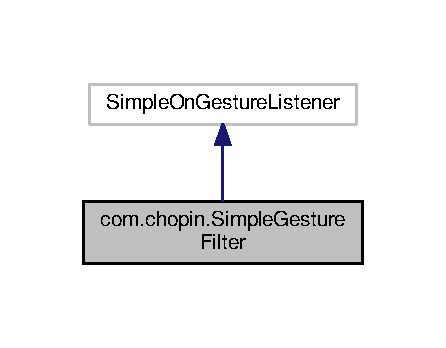
\includegraphics[width=214pt]{classcom_1_1chopin_1_1SimpleGestureFilter__inherit__graph}
\end{center}
\end{figure}


Collaboration diagram for com.\+chopin.\+Simple\+Gesture\+Filter\+:
\nopagebreak
\begin{figure}[H]
\begin{center}
\leavevmode
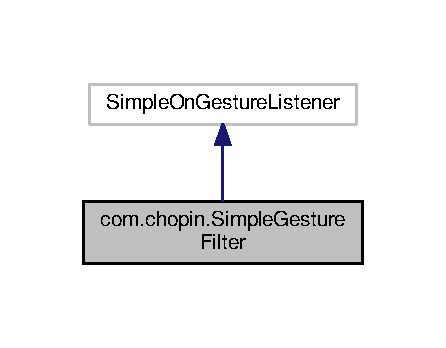
\includegraphics[width=214pt]{classcom_1_1chopin_1_1SimpleGestureFilter__coll__graph}
\end{center}
\end{figure}
\subsection*{Classes}
\begin{DoxyCompactItemize}
\item 
interface {\bfseries Simple\+Gesture\+Listener}
\end{DoxyCompactItemize}
\subsection*{Public Member Functions}
\begin{DoxyCompactItemize}
\item 
\hypertarget{classcom_1_1chopin_1_1SimpleGestureFilter_af3ce91f83615f801a7a5a4d4992ca9b0}{}{\bfseries Simple\+Gesture\+Filter} (Activity context, Simple\+Gesture\+Listener sgl)\label{classcom_1_1chopin_1_1SimpleGestureFilter_af3ce91f83615f801a7a5a4d4992ca9b0}

\item 
\hypertarget{classcom_1_1chopin_1_1SimpleGestureFilter_aa0f6b80bd7046a78170aa4ef7e1d6f4d}{}void {\bfseries on\+Touch\+Event} (Motion\+Event event)\label{classcom_1_1chopin_1_1SimpleGestureFilter_aa0f6b80bd7046a78170aa4ef7e1d6f4d}

\item 
\hypertarget{classcom_1_1chopin_1_1SimpleGestureFilter_a93214a56e0e5083e21374a4ea679d86a}{}void {\bfseries set\+Mode} (int m)\label{classcom_1_1chopin_1_1SimpleGestureFilter_a93214a56e0e5083e21374a4ea679d86a}

\item 
\hypertarget{classcom_1_1chopin_1_1SimpleGestureFilter_a07c13f2f34e3b08451db07b266ab2d8e}{}int {\bfseries get\+Mode} ()\label{classcom_1_1chopin_1_1SimpleGestureFilter_a07c13f2f34e3b08451db07b266ab2d8e}

\item 
\hypertarget{classcom_1_1chopin_1_1SimpleGestureFilter_ab545f0113399137a8788138603caaaa6}{}void {\bfseries set\+Enabled} (boolean status)\label{classcom_1_1chopin_1_1SimpleGestureFilter_ab545f0113399137a8788138603caaaa6}

\item 
\hypertarget{classcom_1_1chopin_1_1SimpleGestureFilter_a6aafbd67deec72e61e2cc62d34248182}{}void {\bfseries set\+Swipe\+Max\+Distance} (int distance)\label{classcom_1_1chopin_1_1SimpleGestureFilter_a6aafbd67deec72e61e2cc62d34248182}

\item 
\hypertarget{classcom_1_1chopin_1_1SimpleGestureFilter_a56e98209542bab7e32fb0e4765aab019}{}void {\bfseries set\+Swipe\+Min\+Distance} (int distance)\label{classcom_1_1chopin_1_1SimpleGestureFilter_a56e98209542bab7e32fb0e4765aab019}

\item 
\hypertarget{classcom_1_1chopin_1_1SimpleGestureFilter_a901bae4f567ddc63081aa492c1f9a977}{}void {\bfseries set\+Swipe\+Min\+Velocity} (int distance)\label{classcom_1_1chopin_1_1SimpleGestureFilter_a901bae4f567ddc63081aa492c1f9a977}

\item 
\hypertarget{classcom_1_1chopin_1_1SimpleGestureFilter_a147e3bdf932d1452c54f61c6039d486a}{}int {\bfseries get\+Swipe\+Max\+Distance} ()\label{classcom_1_1chopin_1_1SimpleGestureFilter_a147e3bdf932d1452c54f61c6039d486a}

\item 
\hypertarget{classcom_1_1chopin_1_1SimpleGestureFilter_a808f7f24037e8696afa446691deeb8d6}{}int {\bfseries get\+Swipe\+Min\+Distance} ()\label{classcom_1_1chopin_1_1SimpleGestureFilter_a808f7f24037e8696afa446691deeb8d6}

\item 
\hypertarget{classcom_1_1chopin_1_1SimpleGestureFilter_a094e37dde168c3b7d3c66fc8a9de01a6}{}int {\bfseries get\+Swipe\+Min\+Velocity} ()\label{classcom_1_1chopin_1_1SimpleGestureFilter_a094e37dde168c3b7d3c66fc8a9de01a6}

\item 
\hypertarget{classcom_1_1chopin_1_1SimpleGestureFilter_a1f2c523774430ee76285323825a346b0}{}boolean {\bfseries on\+Fling} (Motion\+Event e1, Motion\+Event e2, float velocity\+X, float velocity\+Y)\label{classcom_1_1chopin_1_1SimpleGestureFilter_a1f2c523774430ee76285323825a346b0}

\item 
\hypertarget{classcom_1_1chopin_1_1SimpleGestureFilter_a4dc6a2c2fba9016084f755b6d2ed81d7}{}boolean {\bfseries on\+Single\+Tap\+Up} (Motion\+Event e)\label{classcom_1_1chopin_1_1SimpleGestureFilter_a4dc6a2c2fba9016084f755b6d2ed81d7}

\item 
\hypertarget{classcom_1_1chopin_1_1SimpleGestureFilter_adf6727b617db482e35bc5a5bde56ed44}{}boolean {\bfseries on\+Double\+Tap} (Motion\+Event arg)\label{classcom_1_1chopin_1_1SimpleGestureFilter_adf6727b617db482e35bc5a5bde56ed44}

\item 
\hypertarget{classcom_1_1chopin_1_1SimpleGestureFilter_a6b5c5b72853b24ddd68f10f8d15dea8e}{}boolean {\bfseries on\+Double\+Tap\+Event} (Motion\+Event arg)\label{classcom_1_1chopin_1_1SimpleGestureFilter_a6b5c5b72853b24ddd68f10f8d15dea8e}

\item 
\hypertarget{classcom_1_1chopin_1_1SimpleGestureFilter_abf7b53665fbe2abd3075e42a5700b962}{}boolean {\bfseries on\+Single\+Tap\+Confirmed} (Motion\+Event arg)\label{classcom_1_1chopin_1_1SimpleGestureFilter_abf7b53665fbe2abd3075e42a5700b962}

\end{DoxyCompactItemize}
\subsection*{Static Public Attributes}
\begin{DoxyCompactItemize}
\item 
\hypertarget{classcom_1_1chopin_1_1SimpleGestureFilter_a312d0ab12c4bf31d1b837d5e55da9984}{}static final int {\bfseries S\+W\+I\+P\+E\+\_\+\+U\+P} = 1\label{classcom_1_1chopin_1_1SimpleGestureFilter_a312d0ab12c4bf31d1b837d5e55da9984}

\item 
\hypertarget{classcom_1_1chopin_1_1SimpleGestureFilter_a7f1321fdd2723813ae11e6f769cddc1c}{}static final int {\bfseries S\+W\+I\+P\+E\+\_\+\+D\+O\+W\+N} = 2\label{classcom_1_1chopin_1_1SimpleGestureFilter_a7f1321fdd2723813ae11e6f769cddc1c}

\item 
\hypertarget{classcom_1_1chopin_1_1SimpleGestureFilter_a60f246c8bc01218c0155f2ab6fffdf95}{}static final int {\bfseries S\+W\+I\+P\+E\+\_\+\+L\+E\+F\+T} = 3\label{classcom_1_1chopin_1_1SimpleGestureFilter_a60f246c8bc01218c0155f2ab6fffdf95}

\item 
\hypertarget{classcom_1_1chopin_1_1SimpleGestureFilter_a82dee6b6cf4984fd74b781ecd3ebf715}{}static final int {\bfseries S\+W\+I\+P\+E\+\_\+\+R\+I\+G\+H\+T} = 4\label{classcom_1_1chopin_1_1SimpleGestureFilter_a82dee6b6cf4984fd74b781ecd3ebf715}

\item 
\hypertarget{classcom_1_1chopin_1_1SimpleGestureFilter_a4906d19d6bc0eee19974a446db05d17e}{}static final int {\bfseries M\+O\+D\+E\+\_\+\+T\+R\+A\+N\+S\+P\+A\+R\+E\+N\+T} = 0\label{classcom_1_1chopin_1_1SimpleGestureFilter_a4906d19d6bc0eee19974a446db05d17e}

\item 
\hypertarget{classcom_1_1chopin_1_1SimpleGestureFilter_ac27a4d99dc8996ee9286e3bab0789d28}{}static final int {\bfseries M\+O\+D\+E\+\_\+\+S\+O\+L\+I\+D} = 1\label{classcom_1_1chopin_1_1SimpleGestureFilter_ac27a4d99dc8996ee9286e3bab0789d28}

\item 
\hypertarget{classcom_1_1chopin_1_1SimpleGestureFilter_ab80ed42868d3f0717aa033bca61c8bfc}{}static final int {\bfseries M\+O\+D\+E\+\_\+\+D\+Y\+N\+A\+M\+I\+C} = 2\label{classcom_1_1chopin_1_1SimpleGestureFilter_ab80ed42868d3f0717aa033bca61c8bfc}

\end{DoxyCompactItemize}


\subsection{Detailed Description}
Created by mason on 4/14/2015. 

The documentation for this class was generated from the following file\+:\begin{DoxyCompactItemize}
\item 
Simple\+Gesture\+Filter.\+java\end{DoxyCompactItemize}

\hypertarget{classcom_1_1chopin_1_1Song}{}\section{com.\+chopin.\+Song Class Reference}
\label{classcom_1_1chopin_1_1Song}\index{com.\+chopin.\+Song@{com.\+chopin.\+Song}}
\subsection*{Public Member Functions}
\begin{DoxyCompactItemize}
\item 
\hypertarget{classcom_1_1chopin_1_1Song_a5d23605b2530d06b9a3e51b4b429b081}{}{\bfseries Song} (long song\+I\+D, String song\+Title, String song\+Artist)\label{classcom_1_1chopin_1_1Song_a5d23605b2530d06b9a3e51b4b429b081}

\item 
\hypertarget{classcom_1_1chopin_1_1Song_aee53bad2ed0d8f2c8fa0f029e87eb261}{}long {\bfseries get\+I\+D} ()\label{classcom_1_1chopin_1_1Song_aee53bad2ed0d8f2c8fa0f029e87eb261}

\item 
\hypertarget{classcom_1_1chopin_1_1Song_a1a45e519b0bef1472fba21bd4642a165}{}String {\bfseries get\+Title} ()\label{classcom_1_1chopin_1_1Song_a1a45e519b0bef1472fba21bd4642a165}

\item 
\hypertarget{classcom_1_1chopin_1_1Song_acd2e913b6bda13bb83ec102b8367a348}{}String {\bfseries get\+Artist} ()\label{classcom_1_1chopin_1_1Song_acd2e913b6bda13bb83ec102b8367a348}

\item 
\hypertarget{classcom_1_1chopin_1_1Song_a8770d3de8fb394dc97dc8f89093765eb}{}\hyperlink{classcom_1_1chopin_1_1Song}{Song} {\bfseries next\+Song} ()\label{classcom_1_1chopin_1_1Song_a8770d3de8fb394dc97dc8f89093765eb}

\end{DoxyCompactItemize}


\subsection{Detailed Description}
Created by branden on 2/27/15. 

The documentation for this class was generated from the following file\+:\begin{DoxyCompactItemize}
\item 
Song.\+java\end{DoxyCompactItemize}

\hypertarget{classcom_1_1chopin_1_1SongAdapter}{}\section{com.\+chopin.\+Song\+Adapter Class Reference}
\label{classcom_1_1chopin_1_1SongAdapter}\index{com.\+chopin.\+Song\+Adapter@{com.\+chopin.\+Song\+Adapter}}


Inheritance diagram for com.\+chopin.\+Song\+Adapter\+:
\nopagebreak
\begin{figure}[H]
\begin{center}
\leavevmode
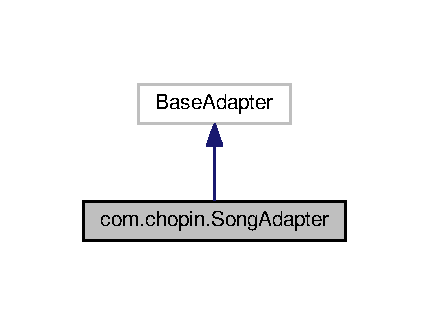
\includegraphics[width=206pt]{classcom_1_1chopin_1_1SongAdapter__inherit__graph}
\end{center}
\end{figure}


Collaboration diagram for com.\+chopin.\+Song\+Adapter\+:
\nopagebreak
\begin{figure}[H]
\begin{center}
\leavevmode
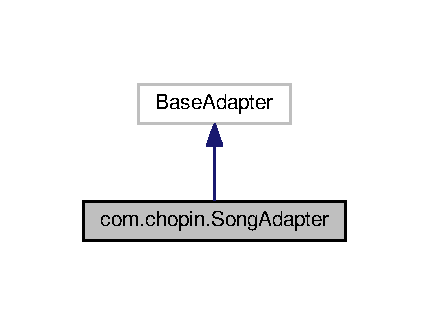
\includegraphics[width=206pt]{classcom_1_1chopin_1_1SongAdapter__coll__graph}
\end{center}
\end{figure}
\subsection*{Public Member Functions}
\begin{DoxyCompactItemize}
\item 
\hypertarget{classcom_1_1chopin_1_1SongAdapter_a8cd1312807a8d367b6ceddc02120d1f4}{}{\bfseries Song\+Adapter} (Context c, Array\+List$<$ \hyperlink{classcom_1_1chopin_1_1Song}{Song} $>$ the\+Songs)\label{classcom_1_1chopin_1_1SongAdapter_a8cd1312807a8d367b6ceddc02120d1f4}

\item 
\hypertarget{classcom_1_1chopin_1_1SongAdapter_aa520e846979d66d2649172dd2c296e4e}{}int {\bfseries get\+Count} ()\label{classcom_1_1chopin_1_1SongAdapter_aa520e846979d66d2649172dd2c296e4e}

\item 
\hypertarget{classcom_1_1chopin_1_1SongAdapter_a1748f00cb93784996f310436ea7c307e}{}Object {\bfseries get\+Item} (int arg0)\label{classcom_1_1chopin_1_1SongAdapter_a1748f00cb93784996f310436ea7c307e}

\item 
\hypertarget{classcom_1_1chopin_1_1SongAdapter_aab43309778c8eda35828b4302379a497}{}long {\bfseries get\+Item\+Id} (int arg0)\label{classcom_1_1chopin_1_1SongAdapter_aab43309778c8eda35828b4302379a497}

\item 
\hypertarget{classcom_1_1chopin_1_1SongAdapter_a344c61b360d6f749574fc56ad3a96ba0}{}View {\bfseries get\+View} (int position, View convert\+View, View\+Group parent)\label{classcom_1_1chopin_1_1SongAdapter_a344c61b360d6f749574fc56ad3a96ba0}

\end{DoxyCompactItemize}


\subsection{Detailed Description}
Created by branden on 2/27/15. 

The documentation for this class was generated from the following file\+:\begin{DoxyCompactItemize}
\item 
Song\+Adapter.\+java\end{DoxyCompactItemize}

%--- End generated contents ---

% Index
\backmatter
\newpage
\phantomsection
\clearemptydoublepage
\addcontentsline{toc}{chapter}{Index}
\printindex

\end{document}
